\documentclass[12pt]{report}

% Packages
\usepackage[english]{babel}
\usepackage[utf8]{inputenc}
\usepackage{graphicx}
\usepackage{fancyhdr}
\usepackage{acro}
\usepackage{amsmath}
\usepackage{amssymb}
\usepackage{amsfonts}
\usepackage{float}
\usepackage{hyperref}
\usepackage{url}
\usepackage{listings}
\usepackage{color}
\usepackage{verbatim}
\usepackage{fancyvrb}
\usepackage[T1]{fontenc}
\usepackage{minted}
\usepackage[language=english]{lipsum} % For dummy text
\usepackage{titlesec}
\usepackage{longtable}
\usepackage{geometry}
\setlength{\headheight}{14.499998pt}
\setlength{\topmargin}{-2.49998pt}
\setcounter{tocdepth}{1}
\titleformat{\chapter}[display]
  {\normalfont\bfseries}{}{0pt}{\Large}

\newcommand\todo[1]{{\vspace{4mm}\noindent\color{red}\textbf{TODO: }#1\vspace{2mm}}}
\newcommand{\javaf}{\mintinline[breakanywhere]{java}}

\lstdefinestyle{yaml}{
     basicstyle=\color{blue}\footnotesize,
     rulecolor=\color{black},
     string=[s]{'}{'},
     stringstyle=\color{blue},
     comment=[l]{:},
     commentstyle=\color{black},
     morecomment=[l]{-}
 }

\hypersetup{
  colorlinks    = true, %Colours links instead of ugly boxes
  urlcolor      = blue, %Colour for external hyperlinks
  linkcolor     = blue, %Colour of internal links
  citecolor     = red %Colour of citations
}

\newcommand{\toclink}{\hyperlink{toc}{\Large\bfseries\thesection\quad}}

% Format for the section headings

% Is it possible for the command below to go the clicked section instead of just to the table of content?
% That command still just send me to the to top of toc and not the clicked section

\titleformat{\section}[block]
{\normalfont\Large\bfseries}{\toclink}{0em}{}

\pagestyle{fancy}
\fancyhf{}
\rhead{Morten Lund Jakobsen}
\cfoot{University of Southern Denmark}
\rfoot{\thepage{}/\pageref{lastpage}}
\lfoot{}
\renewcommand{\headrulewidth}{0.5pt}
\renewcommand{\footrulewidth}{0.5pt}

% Acronyms
\DeclareAcronym{test}{
	short = ST,
	long = Something Test,
}
\DeclareAcronym{CI/CD}{
	short = CI/CD,
	long = Continuous Integration/Continuous Deployment,
}
\DeclareAcronym{CTF}{
	short = CTF,
	long = Capture The Flag,
}
\DeclareAcronym{CVE}{
	short = CVE,
	long = Common Vulnerabilities and Exposures,
}
\DeclareAcronym{CLI}{
	short = CLI,
	long = Command Line Interface,
}
\DeclareAcronym{API}{
	short = API,
	long = Application Programming Interface,
}
\DeclareAcronym{HTTP}{
	short = HTTP,
	long = Hyper Text Transfer Protocol,
}
\DeclareAcronym{HTTPS}{
	short = HTTPS,
	long = Hyper Text Transfer Protocol Secure,
}
\DeclareAcronym{SSH}{
	short = SSH,
	long = Secure Shell,
}
% URL - Uniform Resource Locator
\DeclareAcronym{URL}{
	short = URL,
	long = Uniform Resource Locator,
}
\DeclareAcronym{DNS}{
	short = DNS,
	long = Domain Name System,
}
\DeclareAcronym{IP}{
	short = IP,
	long = Internet Protocol,
}
\DeclareAcronym{OS}{
	short = OS,
	long = Operating System,
}
\DeclareAcronym{VM}{
	short = VM,
	long = Virtual Machine,
}
\DeclareAcronym{Git}{
	short = Git,
	long = Global Information Tracker,
}
\DeclareAcronym{RESTAPI}{
	short = REST API,
	long = Representational State Transfer Application Programming Interface,
}
\DeclareAcronym{CS}{
	short = CS,
	long = Computer Science,
}
\DeclareAcronym{devops}{
	short = DevOps,
	long = Development and Operations,
}
\DeclareAcronym{SSL}{
	short = SSL,
	long = Secure Sockets Layer,
}
% CA - Certificate Authority
\DeclareAcronym{CA}{
	short = CA,
	long = Certificate Authority,
}
% RSA - Rivest-Shamir-Adleman
\DeclareAcronym{RSA}{
	short = RSA,
	long = Rivest-Shamir-Adleman,
}
% CSR - Certificate Signing Request
\DeclareAcronym{CSR}{
	short = CSR,
	long = Certificate Signing Request,
}
% x509 - Standard for Public Key Certificates
\DeclareAcronym{x509}{
	short = x509,
	long = Standard for Public Key Certificates,
}
% NAT - Network Address Translation
\DeclareAcronym{NAT}{
	short = NAT,
	long = Network Address Translation,
}
% CN - Common Name
\DeclareAcronym{CN}{
	short = CN,
	long = Common Name,
}
% FQDN - Fully Qualified Domain Name
\DeclareAcronym{FQDN}{
	short = FQDN,
	long = Fully Qualified Domain Name,
}
% YAML - YAML Ain't Markup Language
\DeclareAcronym{YAML}{
	short = YAML,
	long = YAML Ain't Markup Language,
}
% SDK - Software Development Kit
\DeclareAcronym{SDK}{
	short = SDK,
	long = Software Development Kit,
}
% AAU - Aalborg University
\DeclareAcronym{AAU}{
	short = AAU,
	long = Aalborg University,
}
% SDU - University of Southern Denmark
\DeclareAcronym{SDU}{
	short = SDU,
	long = University of Southern Denmark,
}
% IaaS - Infrastructure as a Service
\DeclareAcronym{IaaS}{
	short = IaaS,
	long = Infrastructure as a Service,
}
% DeiC - Danish e-Infrastructure Consortium
\DeclareAcronym{DeiC}{
	short = DeiC,
	long = Danish e-Infrastructure Consortium,
}
% GCP - Google Cloud Platform
\DeclareAcronym{GCP}{
	short = GCP,
	long = Google Cloud Platform,
}
% AWS - Amazon Web Services
\DeclareAcronym{AWS}{
	short = AWS,
	long = Amazon Web Services,
}
% Azure - Microsoft Azure
\DeclareAcronym{Azure}{
	short = Azure,
	long = Microsoft Azure,
}
% vCPU - Virtual Central Processing Unit
\DeclareAcronym{vCPU}{
	short = vCPU,
	long = Virtual Central Processing Unit,
}
% RAM - Random Access Memory
\DeclareAcronym{RAM}{
	short = RAM,
	long = Random Access Memory,
}
% DDC - De Danske Cybermesterskaber
\DeclareAcronym{DDC}{
	short = DDC,
	long = De Danske Cybermesterskaber,
}
% GUAC - Apache Guacamole
\DeclareAcronym{GUAC}{
	short = GUAC,
	long = Apache Guacamole,
}
% Golang - Go Programming Language
\DeclareAcronym{Golang}{
	short = Go,
	long = Go Programming Language,
}
% RDP - Remote Desktop Protocol
\DeclareAcronym{RDP}{
	short = RDP,
	long = Remote Desktop Protocol,
}
% gRPC - gRPC Remote Procedure Call
\DeclareAcronym{gRPC}{
	short = gRPC,
	long = gRPC Remote Procedure Call,
}
% HAAUKINS - HAAUKINS
\DeclareAcronym{HAAUKINS}{
	short = \javaf{HAAUKINS},
	long = HAAUKINS,
}
% TLD - Top Level Domain
\DeclareAcronym{TLD}{
	short = TLD,
	long = Top Level Domain,
}
% CI - Continuous Integration
\DeclareAcronym{CI}{
	short = CI,
	long = Continuous Integration,
}
% CD - Continuous Deployment
\DeclareAcronym{CD}{
	short = CD,
	long = Continuous Deployment,
}
% CSV - Comma Separated Values
\DeclareAcronym{CSV}{
	short = CSV,
	long = Comma Separated Values,
}
% TOS - Terms of Service
\DeclareAcronym{TOS}{
	short = TOS,
	long = Terms of Service,
}
% Ucloud - Ucloud
\DeclareAcronym{Ucloud}{
	short = Ucloud,
	long = Ucloud,
}


\begin{document}

\begin{titlepage}

	\begin{center}
		
\includegraphics[scale=0.7]{images/SDU_logo.png}
	\end{center}

	\thispagestyle{fancy}

	\center

	\textsc{\large University of Southern Denmark} \\
	\vspace{0.3cm}

	\textsc{\large Masters Thesis}

	\vspace{0.3cm}

	\noindent\makebox[\linewidth]{\rule{\linewidth}{1.2pt}}
	\textsc{\textbf{Empowering DevOps Security: Capture the Flag Challenge in Development and Operations}}
	\noindent\makebox[\linewidth]{\rule{\linewidth}{1.2pt}}

	\vspace{0.5in}

	\begin{minipage}{0.48\textwidth}
		\begin{flushleft}
			\textit{Student:} \\
			Morten Lund Jakobsen \\
			Mojak18@student.sdu.dk
		\end{flushleft}
	\end{minipage}
	\begin{minipage}{0.48\textwidth}
		\begin{flushright}
			\textit{Advisors:} \\
			Jacopo Mauro \\
			mauro@imada.sdu.dk \\
			Macro Peressotti \\
			peressotti@imada.sdu.dk \\
		\end{flushright}
	\end{minipage}

	\vspace{2in}

	\textbf{\large Department of Mathematics and Computer Science} \\

	{\large 1st of June, 2024}
	\thispagestyle{empty}

\end{titlepage}

% \chapter*{Prologue}

\newpage
\hypertarget{toc}{}
\tableofcontents
\newpage
\listoffigures

\begin{abstract}
    I denne afhandling er der blevet undersøgt og udviklet en pipeline som kan bruges til 
    at generere, træne og vise \ac{CTF}'s i et \ac{devops} miljø. Pipelinen 
    er opbygget af 5 forskelle programmer og kan køres lokalt, 
    på computere der har operativ system kali eller ubuntu linux.
    
    Det overordnede mål for denne afhandling var først og fremmest at undersøge, mulighed for at bruge cloud computing 
    til pipeline-infrastrukturen. Derudover at se om et automatiseret virtualiseringsprogram kan bruges til at 
    beværte pipelinen, hvilket på sigt vil gøre det muligt for både brugere og udviklere at håndtere pipelinen og dens ressourcer. 
    Derudover. har det været i fokus at gøre en pipeline tilgængelig for brugeren, sammen med 
    undervisningsmateriale i form af CTF'er, som kan hjælpe brugeren med at forstå pipelinen og samtidig lære om sikkerhed i pipelines.
    
    I denne afhandling er produktet, der er blevet fremstillet, en pipeline.
    Pipelinen kan køres lokalt og opstartes ved bruge at et skript. 
    Fuldføres skriptet uden fejl, vil brugeren blive præsenteret med tre links.
    Disse tre links er til Gitea, Drone og Registry. 
    Disse er de tre programmer som brugeren kan interagere med for at bruge pipelinen,
    og i disse tre programmer er der 4 CTF'er som brugeren kan løse.
    \\
    Udover fremstilling af pipelinen, blevet det også en mulighed at undersøge om "cloud computing"
    kunne anvendes.
    Dette blev undersøgt ved at bruge en platform kaldet Ucloud.Ucloud's maskiner 
    er tilgængelige ved brugen at en SSH forbindelse. På grund af denne begrænsning på 
    Ucloud maskiner, var det ikke muligt at bruge Ucloud som en ressource til at køre infrastrukturen for pipelinen.
    \javaf{HAAUKINS} skulle bruges til at hoste pipelinen og gøre det let for brugerne 
    at intergerer med det udviklede materiale.
    \javaf{HAAUKINS} programmet blev undersøgt og 
    det viste sig, at med den minimale dokumentation og manglede support fra udviklerne, 
    at det ikke var muligt at få haaukins til at køre lokal, og derved ikke have nogen som 
    kontrol over programmet som afhandlingen havde brug for.\\
    I sidste ende kan det konkluderes, at den udviklede pipeline kan køres og startes totalt lokalt, og at brugeren
    kan anvende pipelinen til at løse de tilgængelige \ac{CTF}'er.
\end{abstract}
\begin{abstract}
    This thesis set to investigated and develope a pipeline that can be used to generate, train, and display Capture The Flags (CTFs) in a DevOps environment. 
    The pipeline is composed of 5 different programs and can be run locally on computers with Kali or Ubuntu Linux 
    operating systems.

    The aim goal of this thesis was to investigate if it would be possible 
    to use cloud computing for the pipeline's infrastructure. Secondly, to investigate whether it is possible to use an automated 
    virtualization program to host the pipeline, which effectively allows both the developer to manage the pipeline and its resources,
    and user to interact with it easily. 
    Last but not least, to investigate and develop a pipeline that can be locally accessible to the user, along with developing educational material 
    in the form of CTFs that could be used to enable the user to understand the pipeline while also learning about security in pipelines.

    The result of this thesis is a pipeline where the user can run a simple script. 
    This script will automatically check and verify if all necessary programs are installed. 
    If the script completes without errors, the user will be presented with three links: Gitea, Drone, and Registry. 

    Besides generating a pipeline, the possiblity of using cloud computing was investigated.
    This was explored by using a program called Ucloud.
    Ucloud's machines are only accessible through a SSH connection, 
    it was not possible to use Ucloud as computing power to run the 
    infrastructure for the pipeline, due to this limitation.

    The Haaukins program was intended to host the pipeline and make it easy for users to interact with the pipeline. 
    The Haaukins program was investigated and it turned out that due to minimal documentation and lack of support from the developers,
    it was not possible to run Haaukins locally, and therefore, was the aim of having the program run not achievable.

    Ultimately, it can be concluded that the pipeline can be run locally and that the user can use the pipeline to solve
    the available \ac{CTF}s that are present on the pipeline. 
    It can also be concluded that it was not possible to use Ucloud or Haaukins to host the pipeline.
    
\end{abstract}


\newpage

\chapter{Introduction}
For the last twenty years of software development, software developers have embraced the terminology of \ac{devops}.
\ac{devops} is a set of practices that combines software development (Dev) and IT operations (Ops). 
It aims to shorten the systems development life cycle and provide \ac{CI} and \ac{CD} with high software quality. 
\ac{devops} is complementary with Agile software development; several DevOps aspects came from Agile methodology. 

\ac{devops} started back in the early 21st century, and was first adapted by Amazon led by a man named Verner Vogels.
Vogels is considered the father of \ac{devops} by many software developers and IT professionals. From his perspective, 
he saw the need for a new way of working, where the development and operations teams would work together to
deliver software faster and more reliably. Instead of still using old ways of creating software 
like the waterfall model, where once a stage has been surpassed it's either impossible or very expensive to go back and change something.
\cite{devops}

Today, the new approach to software development, testing, and deployment has evolved into a structured process known as a pipeline. 
A pipeline consists of a series of automated steps that are executed whenever a developer merges code into a production branch or any 
branch connected to the pipeline, such as a test branch. While there are various ways to implement pipelines, the most common method involves 
using \ac{CI/CD} tools.

Nearly all software development companies today utilize some form of pipeline. These pipelines often contain sensitive information, 
including credentials, tokens, and other confidential data needed to deploy software to servers, cloud providers, or container registries. 
Due to the necessity of having access to these credentials and sensitive information, pipelines have become attractive targets for attackers. 
If an attacker gains access to a pipeline, they can potentially compromise the company's entire infrastructure.
Given this security risk, it is crucial to educate developers about potential security gaps in their pipelines and the bad practices they should avoid. 

In this thesis the focus is \ac{devops}. \ac{devops} introduces a new way of working using 
\ac{CI/CD}. Even though practices of \ac{CI/CD} are important, they are not the primary focus in this thesis. 
\ac{CI/CD} is a well-established practice, and numerous tools and platforms are available to facilitate its implementation.

The primary focus of this thesis will be, the creation of a pipeline and \ac{CTF} challenges that 
will help inform and educate developers about the security risks associated with pipelines. 
Currently, there a small amount of training material or \ac{CTF}'s to educate developers on securing their pipelines.
As of this reason, this project proposes the creation of a pipeline using open-source tools, 
designed with a set of challenges aimed towards improving pipeline security knowledge. 
Additionally, it is necessary to have a computational platform where this pipeline can be deployed, such as cloud computing.

HAAUKINS, an automated virtualization platform used by \ac{DDC} for hosting \ac{CTF} events, will be utilized to deploy and host these challenges. 
This platform will provide a practical environment for developers to learn and practice secure pipeline practices. 
Lastly, all this infrastructure will need some kind of computational power or cloud provider to run on. As 
\ac{SDU} is part of \ac{Ucloud}, a computational cloud provider, this thesis will explore the 
possibility of deploying the pipeline on \ac{Ucloud}.

At the end of the thesis, a pipeline locally deployable with multiple \ac{CTF}s on the pipeline was achieved.
Also the thesis concludes that the use of \ac{HAAUKINS} and \ac{Ucloud} was not possible.
Through GameSS\cite{gamess} it was possible to have
the pipeline tested by a group called Brunnerne. Brunnerne is a local group of people from Odense and \ac{SDU}, that are
enthusiastic about \ac{CTF}. This testing provided valuable feedback on the pipeline as the group were appreciated 
by the existing new form of \ac{CTF} challenges but expressed a desire to see more challenges with a more technical focus.

The structure of the thesis is as follows:
\begin{itemize}
    \item Chapter 1 \javaf{State of the art}, An explanation of tools and other pipeline technologies that are out there.
    \item Chapter 2 \javaf{Techninal Implementation} - The thesis has two implementations. One pipeline that was created with a remote server, and 
    one that is totally localized.
    \item Chapter 3 \javaf{HAAUKINS and Ucloud} - In this chapter the two platforms are introduced and explained.
    \item Chapter 4 \javaf{Discussion} - In the discussion there will be a focus on the challenge faced during the projects.
    Also there will be a reflection and a future work discussion.
    \item Chapter 5 \javaf{Conclusion} - An overall conclusion that reflects on the goals of the project.
\end{itemize}
The source code for this project can be found online at \url{https://git.imada.sdu.dk/mojak18/Empowering_DevOps_Security}

\chapter{State of the Art}

\section*{\ac{CI/CD}}
In this chapter, the discussion will focus on the tools and technologies employed in this pipeline. 
Furthermore, other pipeline projects or Capture The Flag (CTF) challenges related to DevOps security will be introduced. 
Before diving into the tools utilized in this pipeline, 
the concept of Continuous Integration (\ac{CI}) and Continuous Deployment (\ac{CD}) will be introduced.

While \ac{CI} and \ac{CD} are distinct acronyms, they are often combined into one term because they are closely related and commonly occur together.
Continuous Integration (\ac{CI}) involves the continuous integration of code, where a set of practices, often automated, 
are implemented to integrate code changes. The term "continuous" in \ac{CI} refers to the ongoing nature of these practices 
rather than the code integration never stopping. \ac{CI} facilitates quicker feedback, 
enabling developers to observe their code in action promptly, making it easier to identify and rectify bugs and errors. 
The adoption of \ac{CI} doesn't necessarily mandate the use of sophisticated tools or pipelines; 
it simply promotes project agility and responsiveness to changes.\\
Continuous Deployment (\ac{CD}) is closely tied to \ac{CI}, as most software, when created, is ultimately exposed 
to users in some form, necessitating deployment. Thus, \ac{CD} complements \ac{CI}, ensuring that software changes 
are efficiently deployed and made available to users.\cite{duvall2007continuous}

The adoption of Continuous Integration and Continuous Deployment (\ac{CI/CD}) 
typically involves the implementation of a pipeline. A pipeline comprises a series of automated 
processes executed in a predefined sequence. It serves to automate tasks such as building, testing, and deploying software.\\
Constructing a pipeline entails utilizing a set of tools to establish an integrated infrastructure.
A pipeline can be as simple as a single script or as complex as a series of scripts orchestrated by a pipeline platform.\\
The tools discussed in this section are specifically those employed in the pipeline for this project. 
Notably, Ngrok, as discussed in Section \ref{sec:ngrok}, is the only tool not utilized in the final pipeline. 
However, its inclusion in this section is warranted as it played a role in addressing 
challenges encountered during the development of the remote pipeline (Section \ref{sec:pipeline_remote}) which not either in use.

\section{Tools}
\label{sec:tools}
\subsection{Docker}
\label{sec:docker}
Docker plays a pivotal role in this project, serving as an integral tool. 
It offers a clean and efficient means of running instances that essentially 
need to be isolated once they have completed their execution. 
This allows for the encapsulation of the machines or infrastructure used for the \ac{CTF} within Docker images, 
which can then be shared with other systems. When these images are executed on those systems, the expectation is to achieve consistent outcomes.

\subsubsection{What is Docker?}
Docker\cite{docker-docs} is an open platform used for developing, shipping, and running applications. 
It utilizes containers, which are isolated environments for running specific applications. 
Containers are lightweight and encapsulate everything needed for an application to run, 
eliminating the need for the host machine to have specific dependencies installed

\begin{figure}[h]
    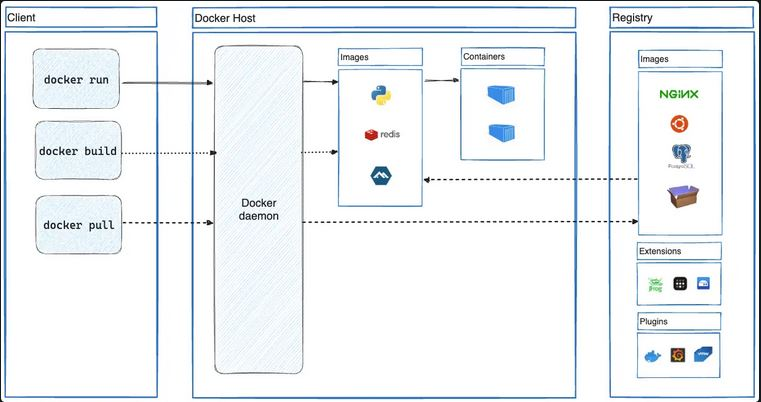
\includegraphics[scale=.7]{images/Docker-architecture.jpg}
    \caption{Docker architecture\cite{docker-docs}}
    \label{fig:docker_architecture}
\end{figure}

The architecture of docker is client-server. 
As seen in figure \ref{fig:docker_architecture} Docker consist of mostly 3 parts; client, daemon (host) and the registry.
The client is the \ac{CLI} which is used as an intermediary to communicate with the daemon. 
The daemon handles everything related to the containers, like building, running, and distributing them.
When images are not stored locally on a users machine or server, they are fetched from the registry.
The registry is a place where images are stored and can be fetched from. There is a many 
authorized registries, but the most common one is Docker Hub.\cite{dockerhub}\\
\paragraph{\textbf{What is a container?}}
A container\cite{docker-concepts} is an isolated process. 
That means that it's a process that runs on a host machine, but it's isolated from the host machine.
Containers can also be described as a lightweight \ac{VM}. Containers are also isolated from each other, but they share the same kernel.
Therefore containers act like components in a bigger project, meaning if a user wants to run a web-application, he or she might need a frontend, database, \ac{API}, etc.
All these things can be isolated from each other, but still have the ability to communicate with each other.
\paragraph{\textbf{What is an image?}}
A container is only as powerful as it's configuration, and for configuring a containers,
Docker uses images\cite{docker-concepts}.\\
Images are the configuration of the container.
They are used to create containers. Images are read-only, meaning that they can not be changed once build.
To change an image, one would to rebuild it from scratch.
For Docker to work, the parts has to work together in harmony. The client sends a request to the daemon, which then executes the request.
If the image isn't stored locally it fetches it or builds it. Once an image is locally present and complete the daemon  
will create a container from the image.
When using the Docker CLI things can quickly become complicated, but with the help of \javaf{docker-compose}, things can be simplified.
\subsubsection{\javaf{docker-compose}}
Docker compose is a tool for running multi-container applications. With the help of \ac{YAML}\cite{YAML}
and a configuration file name \javaf{docker-compose.yml}, it is possible to define services to run.
The docker compose\cite{docker-compose} application model consist of the main 3:
\begin{itemize}
    \item \javaf{Services} is a definition of a containerized application or components of an application. For the Docker compose file,
    this is where the definition of the services that going to be spawn that make the \javaf{docker-compose} file a multiple container application.
    \item \javaf{Networks} is a definition of a virtual network that containers can connect to, in order to communicate with each other.
    If no network is specified, the containers will be connected to the default network. In Docker compose it is possible for 
    containers via Docker internal \ac{DNS} to communicate with each other. 
    This means that even though that IP's might change, the containers can find and communicate with another container through it \ac{DNS} record.
    \item \javaf{Volumes} are a way to persist data generated by containers or share data between containers and the host system. 
\end{itemize}
When combining these three elements, it is possible create a multi-container application. The \javaf{docker-compose} file is a 
\ac{YAML} file that defines the services, networks, and volumes that is going to spawned. Once a developer
has defined everything needed in the \javaf{docker-compose} file, the multi-container application 
can be spawned with a single command, \javaf{docker-compose up}. As there can be many ways to define a \javaf{docker-compose} file, 
we'll wait until section \ref{sec:technical_implementation} to see the \javaf{docker-compose} file that is used in this project.
\newpage

\begin{itemize}
    \item First: Gitea is an open source project and is there subjective to changes at any time. For this project,
    I need to ensure that the end result is the same as when I started the project. 
    To circumvent this, the base image of Gitea is chosen to be version 1.16.5. Now why this version? 
    Based some testing it seems that most of the API admin options are unavailable in version later than 1.19.0. Version between 1.16.5 and 1.19.0
    have changes which impacts the use of admin API options.
    Using the version 1.16.5 Docker image esnure that even though long time developing this project, the base image stay the same and 
    the end result will be same as when i started the project, and when the user pulls the image.
    \item Second: The configuration of Gitea needs to be static. When Gitea is installed, it will prompt the installer of Gitea 
    to specify what that person wants. This information will be stored in a special file called app.ini. This file is 
    used by Gitea to configure itself\ref{fig:gitea_app_ini_remote}. The rest of the app.ini file for this project
    can be found the source code of the project under Gitea/app.ini.
    \item Third: Users needs to be created at initialization, so that when the user start the image via docker-compose. 
    The database is already populated with users, and the user can start using the service right away.
    This is done with python3\cite{python} script which 
    post users to the database via a \ac{RESTAPI}, with admin credentials.
\end{itemize}

\subsection{Drone problems}
\label{sec:discussion-drone}

\subsubsection{Deployment on drone}
The newest version of the Drone server uses Oauth2 to authenticate user account to the server.
This means that another entity, such as gitea authenticates user to the Drone server. This is done by
setting up a Oauth2 application in gitea, and then using the client id and client secret to authenticate
the user to the Drone server. On the Drone official website, it states that it is not recommend to deploy 
Drone with docker-compose, because of the potential network issues that might arise.
\paragraph{Problem 1, integration with gitea over OAuth2}
Other than starting out figuring out how to run Drone, I had to figure out how to integrate it with gitea.
Now later version of Drone, had its own database of users and therefore didn't have to rely on gitea for authentication.
Now this means that before being able to run Drone runners to execute pipeline, the user that wish to use Drone,
needs to authenticate with the gitea server, and post a access token to the gitea server. Essentially the user needs a token 
when is used to authenticate with the gitea server.
Now the authentication process is not a problem, the Drone CI/CD documentation is very specific about how to do it and if done 
correctly it'll work fine.
Now the big problem is posting the token to the gitea server. The gitea server will not accept the token, being posted over http connection,
and it refusing the connection. 
Since Drone need to make it's access token available to the gitea server, it needs to be able to post it to the gitea server.
The problem can be solved by using a proxy or a https connection on the gitea server, but that is not a viable solution.

\paragraph{Problem 2, Advertised problem by Drone}
Now the is linked to the first problem and is about the network aspect of Drone.
The authentication of the user is done in the browser. When that is done Drone obviously needs to be able to communicate with the gitea server.
Now the problem, and im not sure how docker compose works in this part, but what I've deciphered from the internet is that 
Drone might not be able to find the gitea server, and post the token to it.

\paragraph{Problem 3, Drone runner}
When the Drone server is operational, it acts as the intermediary connecting the Git server 
and the runners responsible for executing the pipeline. 
To ensure a smooth pipeline execution, it is imperative that the pipeline configuration 
for the Drone server is exceptionally detailed. This configuration should explicitly define 
crucial details such as the software used to manage the Drone server, particularly Docker if the Drone runners 
are tasked with running the pipeline within Docker containers.

Furthermore, the fact that this specification must be written in YAML introduces a 
level of dependency on YAML syntax and indentation. It's important to note that the 
specific syntax and indentation requirements can vary from one software platform to another when defining the structure of the pipeline. 
Therefore, careful attention to these details is vital to ensure accurate and effective pipeline execution.

\subsection{Ngrok}
\label{sec:ngrok}
Ngrok was used is this product to expose the local Gitea server to the internet. This was done to allow remote access to the server.
Ngrok is a multiplatform tunnelling, reverse proxy software that establishes secure tunnels from a public endpoint to a local running network service.
Ngrok acts as a unified ingress platform combining all the components to deliver traffic from local service to the internet. 
Ngrok consolidates together the reverse proxy, load balancer, \ac{API} gateway, firewall, delivery network, DDoS protection and more.\cite{ngrok}

\subsubsection{How does Ngrok work?}
Ngrok is a reverse proxy but there is a little more to it than just that. Ngrok 
works on a global network called the \javaf{Ngrok edge}. At the edge, traffic is accepted from client from the internet 
and then forwarded to the local service.
Unlike traditional proxies Ngrok does not transmit traffic to an upstream application by forwarding IP address. Instead, 
Ngrok is a small piece of software that you run along side a local application. This software will connect to 
the Ngrok edge and will keep the connection open. When a client connects to the Ngrok edge, the edge will forward the
traffic to the local application.
There are four ways of running the client\cite{ngrok-works}.

\begin{itemize}
    \item As a service: Run as a small side process called the Ngrok agent as a
    background \ac{OS} service.
    \item As an interactive \ac{CLI}: Run as the Ngrok agent
    interactively from the command line while developing and testing.
    \item As an \ac{SDK}
    embedded in your app: Included as a small Agent \ac{SDK} library directly into an
    application software that returns a socket-like object. 
    \item As a Kubernetes
    Controller: Run the Ingress Controller in a Kubernetes environment.
\end{itemize}

In this project, the Ngrok agent was run as a service. This was done to ensure that the connection to the Ngrok edge was at all times.

\subsection{Nginx proxy}
\label{sec:nginx}
Nginx is a reverse proxy, serving as the intermediary between the client and the internal network where the application runs. 
It manages the DNS records requested and directs the traffic to the corresponding IP address. 
Consequently, the client is unaware of the application's IP address, knowing only the gateway. This gateway is a docker network gateway.
The client sends a request to the application via HTTPS. 
The proxy forwards this request to the application, which then sends the response back to the proxy. 
This setup adds an extra layer of abstraction, helping to protect the internal network from the outside world.
It also gives the possible to add more infrastructure to the application, such as load balancing, caching, certificates handling and more.\\

\paragraph{Passing a request to a proxied server}
Whenever nginx receives a request, it tries to find the server that the request should be forwarded to.
The server is specified in the \javaf{proxy_pass} directive. The \javaf{proxy_pass} directive is used to specify the server that the request should be forwarded to.\\
Simply what the \javaf{proxy_pass} specification does, is the declaration of the server that the request should be forwarded to.
That can either be a \ac{DNS} record or an \ac{IP} address.\cite{nginx-proxy-3}

\paragraph{Configuring buffers}By default NGINX buffers responses from upstream servers.
A response is stored in the internal buffers and is not sent to
the client until the whole response is received. Buffering helps to optimize performance with slow clients, 
which can waste upstream servers time if the response is passed from NGINX to the client synchronously. 
However, when buffering is enabled, NGINX allows the upstream servers to 
process responses quickly, while NGINX stores the responses for as much time as the clients need to download them.\cite{nginx-proxy-3}
The specification of these buffers are noted in the configuration as seen in figure \ref{fig:buffer-config}.
\begin{figure}
    \begin{center}
        \javaf{proxy_buffers $size$ $number$;} \\
        \javaf{proxy_buffer_size $size$;}.
    \end{center}
    \caption{Configuring buffers}
    \label{fig:buffer-config}
\end{figure}
The specific configuration for the this project will be covered in section \ref{sec:pipeline-local-nginx}.

\subsubsection{Docker gateway}
\label{sec:gateway}
For the NGINX reverse proxy to function, it needs a gateway to attach itself to. Here the Docker network is used as the gateway.
The Docker network is a virtual network that is created by Docker. The network is used to connect containers together.
The network is created by the Docker daemon when the first container is created. The network is created with the name \javaf{bridge}.
The bridge network is the default network that is created by Docker.
The bridge network is a \ac{NAT} network that is used to connect the containers to the host.

\subsection{Registry}
\label{sec:registry}
The Drone pipeline when using Docker runner needs a registry to pull and push images to.
The default registry that is used is the Docker hub. Because the future work of the project includes
having the project running on haaukins (Section \ref{sec:haaukins}) which does not have internet when running.
Here in comes a local registry. A local registry will resides as a mirror of Docker Hub, when 
other container which has docker installed is made aware of the local registry, it will pull images from the local registry.
If no internet connection is available, the Drone runners will not be able to pull images from the docker hub. 
How this is solved is either by providing all container with the address of the mirror registry of Docker hub or 
using specific \ac{URL} for the desired images in the pipeline.\\
\paragraph{What is a registry?}
A registry is a storage and content delivery system, holding named Docker images, available in different tagged versions.
The registry is a stateless, highly scalable server side application that stores and let you distribute Docker images.
The registry is open-source, under the Apache 2.0 license. Some of the features of the registry are:

\begin{itemize}
    \item The ability to store images in a central location.
    \item The ability to control access to the images.
    \item The ability to integrate image storage and distribution into the \ac{CI/CD} pipeline.
\end{itemize}

\newpage

\subsection{Certificate}
\label{sec:certificate}
Certificates are used for all websites that run \ac{HTTPS}. 
The certificate is used  to let visitors know that the website is secure.
The certificate has associated cryptographic keys that are used to encrypt the data being transferred between the client and the server.
Futhermore, the certificate might be signed by a \ac{CA} which is a trusted third party.
When a client connects to a website that uses \ac{HTTPS}, the client will check the certificate
to see if it is signed by a trusted \ac{CA}. If the certificate is signed by a trusted \ac{CA}, the client
will trust the website. If the certificate is not signed by a trusted \ac{CA}, the client will get a warning
that the website is secured by a self signed certificate.\\
There are various methods to create a certificate, and no single approach is definitive. 
For this project, a self-signed certificate was created to enable HTTPS connections between all services \cite{self-signed-cert}.


\paragraph{Self signed certificate}
When creating a self signed certificate, access to the server or the proxy that is going to handle the certificate is necessary.
The certificate is created using the openssl command first one will have to create a private key:
\begin{figure}[h]
    \begin{center}
        \javaf{openssl genrsa -out eds.key 2048}
    \end{center}
    \caption{Creating a private key}
    \label{fig:private-key}
\end{figure}
The private key created in figure \ref{fig:private-key} is a RSA key that is 2048 bits long. 
Normally, the private key would be encrypted with a password, but for this project, 
the private key will not be encrypted to avoid the need to enter a password during deployment.
Next, a Certificate Signing Request (CSR) will be created. 
A CSR is an encoded file containing information about the organization requesting the certificate \cite{csr}. 
The CSR is sent to a Certificate Authority (CA) for signing. In this case, the certificate will be self-signed.
\begin{figure}[h]
    \begin{center}
        \javaf{openssl req -key eds.key -new -out eds.csr}
    \end{center}
    \caption{Creating a CSR}
    \label{fig:csr-creation}
\end{figure}
When creating a \ac{CSR}, openssl ask for information to be filled. This information is about the creator of the CSR.
The information that is asked for is:
\begin{itemize}
    \item Country Name (2 letter code) [AU]: 
    \item State or Province Name (full name): 
    \item Locality Name (eg, city): 
    \item Organization Name (eg, company): 
    \item Organizational Unit Name (eg, section): 
    \item Common Name (e.g. server FQDN or YOUR name): 
    \item Email Address:
    \item A challenge password:
    \item An optional company name:
\end{itemize}
\ac{CN} is the domain name which the certificate is going to be used for.
After the private key and \ac{CSR} is created, we can create the certificate. We created the certificate using \javaf{x509} format.\\
\javaf{x509}\cite{x509} is standardized format for public key certificates. What \javaf{x509} certificate provides is the ability
to both create a self signed certificate, but also allow our application to be accessed through \ac{HTTPS}.\\
\begin{figure}[h]
    \begin{center}
    \javaf{openssl x509 \ }\\
    \javaf{-signkey eds.key \ }\\
    \javaf{-in eds.csr \ } \\
    \javaf{-req -days 365 -out eds.crt}
\end{center}
    \caption{Creating a certificate}
    \label{fig:cert-creation}
\end{figure}
The certificate, created by the command seen in figure \ref{fig:cert-creation}, is designed for a single page. 
To support multiple websites under various domains within the same subdomain, 
a certificate endorsed by a Certificate Authority (CA) is required.\\
Having the created certificate signed by 
a CA allows the association of the desired subdomain, enabling an unlimited number of subdomains. 
The initial step involves generating a new private key and self-signing 
an CA certificate, which will be used to endorse the previously created certificate.
Now that a CA certificate called edsCA is created by the command seen in figure \ref{fig:ca-cert}.
edsCA can be used to sign the certificate that was created in figure \ref{fig:cert-creation}.\\
\begin{figure}[h]
    \begin{center}
        \javaf{openssl req -x509 -sha256 -days 1825 \ } \\
        \javaf{-newkey rsa:2048 -keyout edsCA.key -out edsCA.crt}
    \end{center}
    \caption{Creating a CA certificate}
    \label{fig:ca-cert}
\end{figure}
A configuration file, named \javaf{eds.ext}, will be used to add additional information to the certificate. 
The \javaf{eds.ext} file contains the following information:
\begin{figure}[h]
    \begin{center}
        \javaf{basicConstraints=CA:FALSE} \\
        \javaf{extendedKeyUsage=serverAuth} \\
        \javaf{subjectAltName = *.devops.eds}
    \end{center}
    \caption{Data for configuration file for the CA certificate}
    \label{fig:ca-cert-ext}
\end{figure}
\javaf{extendedKeyUsage} is serverAuth because we're going to use ssl/TLS authentication a server.
\javaf{basicConstraints} is set to false because the certificate is not a valid  CA certificate.\\
\javaf{subjectAltName} is the domain name that the certificate is going to be used for.\\\cite{openssl-ext}
\begin{figure}[h]
    \begin{center}
        \javaf{openssl x509 -req -CA edsCA.crt \ } \\
        \javaf{-CAkey edsCA.key -in eds.csr \ } \\
        \javaf{-out eds.crt -days 365 \ } \\
        \javaf{-CAcreateserial -extfile eds.ext}
    \end{center}
    \caption{Signing eds.crt with edsCA.crt}
    \label{fig:sign-cert}
\end{figure}

The command from figure \ref{fig:sign-cert} takes a CSR (eds.csr), signs it using the CA certificate 
(edsCA.crt) and its private key (edsCA.key), and generates a signed certificate 
(eds.crt) valid for 365 days, including any specified extensions from the eds.ext file.\\
This certificate has been signed with the CA certificate, 
meaning that if it is placed in \javaf{/etc/ssl/certs/ca-certificates.crt} on Linux, the system will trust the certificate.

\section{CI/CD CTF Pipeline}
\label{sec:ci-cd-ctf-pipeline}
As this project focuses on the development of a pipeline for the creation and deployment of \ac{CTF} challenges, 
it is essential to understand the available pipeline platforms, that are already out there. 
Even though there may not be an existing pipeline exactly 
like the one being developed, it is still important to understand what other tools can and cannot do. 
In this section, I will briefly some of the pipelines that I consider noteworthy. 
These pipelines have some merits in terms of what I believe a pipeline should be able to do and what it should not do.


\paragraph{CICD-Goat}
\label{par:cicd-goat}
The CICD-Goat\cite{cicd-goat} is one of the other \ac{CTF} pipelines that is out there.
The pipeline is created based on the OWASP Top 10 CI/CD security risk\cite{owasp-cicd-top-10} list.
The pipeline is aimed toward developers, security professionals, and others who are interested in understanding the \ac{CI/CD} pipeline.
The pipeline is constructed with technology of Gitea, Jenkins, Gitlab and Gitlab runners.
The pipeline infrastructure is build inside Docker containers and used localhost to export the website.
It used a local instance of CTFd to host the challenges and report the flag.

The CICD-goat project has a lot of merit in the sense that they focus on real proven scenarios that 
is happening to pipelines in productions settings, anyhow the project uses an old technology in Jenkins. Jenkins 
is a great tool, but in the sense of a modern pipeline and pipeline structure, Jenkins is outdated.

\paragraph{Poursoft}
\label{par:poursoft}
Poursoft is the recent create pipeline for the national \ac{DDC}. It was created by Oliver Nordestgaard
and was used in the national \ac{DDC} 2024. The pipeline utilize many of the same tools as the pipeline for this project.
The pipeline is not open-source and can't be referenced in this project. Although through my work on \ac{DDC} 2024,
I had access to the repository and could see how the pipeline was constructed. The pipeline was constructed with the following tools:
\begin{itemize}
    \item \javaf{Gitea} as the git repository.
    \item \javaf{DroneCI} for the pipeline
    \item \javaf{Ngnix} for a websever and reverse proxy
    \item \javaf{Haaukins} for the deployment of the challenges
\end{itemize}

\paragraph{Tryhackme, Hackthebox, and other commercial projects}
\label{par:tryhackme-hackthebox}
TryHackMe and Hack The Box are both commercial platforms and are not open-source. They require a subscription fee for access.
On TryHackMe\cite{tryhackme}, it is possible to view available challenges without logging into the website. 
TryHackMe offers numerous challenges relevant to pipelines. While not directly focused on pipelines, 
these challenges involve tools commonly used in pipelines, such as Docker, Kubernetes, GitLab, DevSecOps practices, and more.\\
Hack The Box\cite{hackthebox} primarily focuses on the exploitation of machines. After exploring their website, it appears they have a few 
DevOps-related challenges. However, 
the specific focus of these challenges is not clearly indicated, making it difficult to assess their relevance to DevOps Capture The Flag (CTF) events.



\newpage


\chapter{Technical Implementation}
\label{sec:technical_implementation}
This section covers the technical part of the pipeline. There will not be much discussion about 
whether one of the pipeline is better than the other or if the implementation is good or not.
Rather I will reflect and discuss that in 
the discussion section \ref{sec:discussion-pipeline}.
Section \ref{sec:pipeline_remote} is about the remote deployment.
Section \ref{sec:pipeline-local} is about the final pipeline product hence 
the local pipeline and it's local deployment.\\\\
The objective of this pipeline is to provide developers with an environment where they can develop and experiment, 
using a setup akin to the production pipeline. They have the flexibility to integrate their own repositories, 
configurations, and other resources into the pipeline to observe its behavior. This enables them to assess and 
refine their development practices based on the pipeline's performance.

Localized pipelines, although less common nowadays, offer a unique advantage. Unlike pipelines hosted on 
cloud-based virtual environments managed by service providers, a localized pipeline resides directly on the developer's machine. 
This grants developers full access to the pipeline's infrastructure, codebase, and configurations. Such accessibility is invaluable 
considering the prevalent use of pipelines 
in modern development workflows, emphasizing the importance of adhering to secure and efficient practices.
For this project the pipeline is constructed with the components that are described in section \ref{sec:tools}.


\section{Pipeline - Remote}
\label{sec:pipeline_remote}
For the first part of the project there was a major a problem with authenticating user between the Gitea server and 
the Drone server.\\
This problem was solved by using a remote Gitea instance which could be accessed over the internet. This meant that the 
Gitea server would not be run locally on a users machine, but instead on a remote server. The Drone server, Drone runners and everything 
related to the deployment of Drone with be on the users end, hence using the users resources. This is how that deployment worked. It consisted of 
five parts:

\begin{itemize}
    \item Gitea configuration (Docker)
    \item Drone configuration (Docker)
    \item Admin (Python script)
    \item Webhook (Python script)
    \item Request script (Python script)
\end{itemize}
This solution for a pipeline had drawbacks, but that will be discussed in the section \ref{sec:discussion-pipeline}. Here
the sole focus is on how the 
product worked and how it was implemented.

\subsection{Gitea configuration}
The Gitea configuration was first created with the intention of being run locally. However, because of the Oauth2 authenticating problem, 
the Gitea server was moved to a remote server. This meant that, although it was possible to close, delete, and recreate the Gitea server with the same configuration, it was no longer necessary. 
However, this configuration made it easy to restart the server if needed.
For the deployment of the Gitea server, the following command was used:
\begin{figure}
    \begin{center}
        \centering
        \javaf{docker compose up -d}
        \caption{Docker compose command use for remote Gitea}
        \label{fig:docker-compose-remote}
    \end{center}
\end{figure}
The command showed in figure \ref{fig:docker-compose-remote} is the basic command for running Docker compose detached. 
Now behind that command is the docker-compose.yml\cite{docker-compose} file.
The docker-compose.yml file is used to define the configuration of the Gitea server. The file is shown below:
\begin{figure}[h]
    \begin{lstlisting}[style=yaml]
        version: '3'
        networks:
            kv:
                name: kv
                driver: bridge
        services:
            gitea:
                image: kraftvaerket/kv-gitea:latest
                container_name: Gitea
                restart: always
                environment:
                    - USER_UID=1000
                    - USER_GID=1000
                networks:
                    - kv
                ports:
                    - "3000:3000"
    \end{lstlisting}
\caption{docker-compose.yaml file for Gitea}
\label{sec:pipeline_remote_gitea_docker_compose}    
\end{figure}

\begin{itemize}
    \item \textbf{image}: Specifies the Docker image to use for this service, in this case, "kraftvaerket/kv-gitea:latest".
    \item \textbf{container\_name}: Specifies the name of the container, in this case, "Gitea".
    \item \textbf{restart}: Specifies the restart policy for the container, in this case, "always", which means Docker will always restart the container if it stops, regardless of the exit status.
    \item \textbf{environment}: Specifies environment variables to be passed to the container. Here, it sets the user UID and GID to 1000.
    \item \textbf{networks}: Specifies which networks this service should be connected to. In this case, it'sconnected to the "kv" network.
    \item \textbf{ports}: Specifies port mappings between the container and the host. In this case, it maps port 3000 on the host to port 3000 on the container, allowing access to the Gitea application running inside the container.
\end{itemize}
The overall of this docker-compose file is simple and basic since all of the configurations were done in the image itself.
The image used is a custom image created by the author, which 
is pulled from DockerHub. Doing all the configurations 
in the image, creates a more robust image that is more reliant to work on different machines.

This Docker compose file was then run on a \ac{Ucloud} machine which then created the Gitea server. 
To make the Gitea server accessible from the internet with another \ac{URL} than \\
\javaf{http://localhost:3000}, a reverse proxy was used called Ngrok \cite{ngrok}.
Ngrok is attached to the Gitea server by running the software running along side the Gitea server.
For that to be done you need to run the following command:
\begin{figure}[h]
    \begin{center}
        \javaf{ngrok http 3000 https://full-enormous-crow.ngrok-free.app}
    \end{center}
    \caption{Ngrok command}
    \label{fig:ngrok-command} 
\end{figure}

\begin{itemize}
    \item
    \javaf{ngrok}\\Ngrok CLI \\
    \item 
    \javaf{http 3000} \\Ngrok communicates with the Gitea server on port 3000 with the protocol http\\
    \item
    \javaf{https://full-enormous-crow.ngrok-free.app}\\Public \ac{URL} that ngrok provides
\end{itemize}

\subsection{Drone configuration}
For Drone to function, it relies on Gitea for user authentication through OAuth2. 
This means the Gitea server must be running before the Drone server can start. 
Since the Gitea server was running remotely and continuously, the Drone server could be started without any issues.

For the remote solution, it still meant that the Drone server and runners would be running locally.
The drone server is started by running a bash script, that would start the Drone server and runners.
This bash script had several functions
\begin{itemize}
    \item First:
    It checked whether all the necessary programs was installed on the machine. If not, the script would exit.
    \item Second:
    Creating a user, followed by the creation of an Oauth2 Application, for that particular user.
    The user would use these credentials to authenticate Drone with the Gitea server.
    \item Third:
    It spawned all the necessary Docker containers, both the server and the runners.
    \item Fourth:
    A newly created repository had to be activated and only after activation, it 
    was it possible to post secret and other configuration a specific repository.
    The script uses the Drone \ac{API} to activate the repository and add necessary secrets that might be used for a CTF or 
    other part of the pipeline.
    To accomplish this, the script required admin credentials for the Drone server. 
    The process involved the user logging in as an admin on the remote Gitea server, 
    authenticating as an admin on the local Drone server, and then navigating to the admin page to copy the token. 
    This token was then input into the script and used to create configurations and backend components for the Drone server.
\end{itemize}
In figure \ref{sec:pipeline_remote_drone_start_script} a snippet of the bash script is shown.
The entire script can be found in the source code under \javaf{archive/drone/drone.sh}.

\begin{figure}[h]
    \centering
    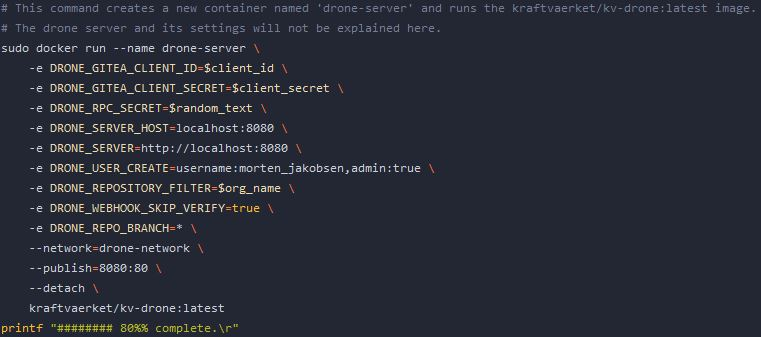
\includegraphics[scale=.69]{images/remote-script-drone.jpg}
    \caption{Drone start script snippet}
    \label{sec:pipeline_remote_drone_start_script}
\end{figure}

The image displays several environmental variables,
you see several environment variables, 
but the two most important ones are; \\ \javaf{DRONE_GITEA_CLIENT_ID} and \javaf{DRONE_GITEA_CLIENT_SECRET}. 
These variables are used to authenticate the Drone server with the Gitea server. 
While the host and RPC secrets for the Drone runners are necessary, 
the authentication credentials for OAuth2 are essential to Drone server to enable it to authenticate itself and the users 
wanting to use it.
To create the OAuth2 credentials 
on the Gitea server, a request script is utilized. This script uses the credentials provided by the user to create an OAuth2 application on the 
Gitea server for that specific user. The command in the script that executes this process is:
\begin{figure}
    \begin{center}
        \javaf{python3 ../requests/request.py $username $password}
    \end{center}
    \caption{Request script command}
    \label{fig:request-script-command}
\end{figure}
The script makes a \javaf{POST} request to the Gitea server and receives the OAuth2 credentials in return.\\
Once the pipeline was deployed and the user was created, webhooks needed to be configured. 
The purpose of the webhook is to listen for any changes in the repositories on the Gitea server. 
When a change is detected, the webhook would sends a request to the Drone server to initiate a pipeline.\\
Since the Gitea server is remote and the Drone server is local, 
an SSH tunnel is required from the remote Gitea server to the local Drone server. 
This is necessary because the Gitea server was hosted on \ac{Ucloud}, and the only way to access the machine is through SSH. 
To establish this connection, a tunnel is created from the Gitea server machine to the machine running the Drone server using the following command:\\
\begin{figure}{h}
    \begin{center}
        \javaf{ssh -Nf -L (GITEA_SERVER_MACHINES PORT):localhost:8080} \\
        \javaf{-i (SSH_KEY_FOR_LOCAL_DRONE_SERVER_MACHINE)}\\
        \javaf{USERNAME@IP_ADDRESS}
    \end{center}
    \caption{SSH tunnel command}
    \label{fig:ssh-tunnel}
\end{figure}
To establish the tunnel, the Gitea server machine needs an SSH key that can access the local machine running the Drone server. 
This is achieved by generating an SSH key on the Gitea server machine and copying the public key to the local machine.\\
Once the connection is established, a Python API on the Gitea server makes POST requests to the Drone server. 
The Gitea webhook sends a POST request to the local Flask API, which then relays the request to the Drone server.\\
\newpage

\section{Pipeline - Local configuration}
\label{sec:pipeline-local}
The localized pipeline is constructed with the components 
that are described in section \ref{sec:tools}, but the components are:

\begin{itemize}
    \item Gitea
    \item Drone
    \item Nginx
    \item Docker
    \item Local registry
    \item Certificate 
\end{itemize}
\subsection{Pipeline deployment}
\label{sec:pipeline-local-deployment}
The deployment of the pipeline is currently only available for certain operating systems. The operating systems that are supported are
\javaf{Ubuntu} and \javaf{Kali}. The deployment is done through a script \javaf{prerun.sh} that is located in the src directive of the repository.
The script consist of two parts. 
\paragraph{Part 1} of the script controls all the prerequisites that are needed for the pipeline to run. Without 
these prerequisites, the pipeline will not be able to run. The prerequisites are:
\begin{itemize}
    \item Package control. The script needs a certain number of specific packages to be installed. The packages are: \javaf{docker},
    \javaf{docker-compose}, \javaf{curl}, \javaf{python3}, \javaf{jq}, and \javaf{openssl}. There are also some packages needed that are not listed, 
    but they are preinstalled on all Ubuntu\cite{ubuntu} and Kali\cite{kali} systems.
    \item Creation of a \javaf{docker network}. This network is where all the containers will be located and communicate over.
    This network is also where the gateway to the reverse proxy is located. Without this network, the user would not be able to communicate with the pipeline.
    \item When the \javaf{docker network} is created, the script will insert a \ac{DNS} record in the 
    \javaf{/etc/hosts} file generic to Ubuntu and Kali systems. This is done so that the user can access the website with a \ac{DNS} record.
    \item Last in the first part of the script is the insertion of the certificate created for 
    the pipeline. The certificate needs to be inserted into the hosts\\
    \javaf{/etc/ssl/certs/ca-certificates.crt} file because the drone runners will use the host volumes for its certificate.
\end{itemize}
The first part of the script ensures that all prerequisites are met. The final command of part 1 initiates the spawning of containers. 
The script uses Docker Compose for this task, and the command used is shown in Figure \ref{fig:docker-compose-localized}.\\
When the first part is complete without error, the script shown in Figure \ref{fig:docker-compose-localized}.
\begin{figure}[h]
    \begin{center}
        \javaf{docker compose --env-file .env up --build -d}
    \end{center}
    \caption{docker compose command to spawn localized pipeline containers}
    \label{fig:docker-compose-localized}
\end{figure}


\paragraph{Second part} of the script waits for the containers to be up and running.
All the commands in the second part of the script is a health check to see if everything is running correctly.
It is also to make the user wait until everything works. Some of the containers depends on other containers, and 
therefore if interacted with before those containers are ready, would mean that there could be a potential error.


\subsection{Gitea}
\label{sec:pipeline-local-gitea}

When Gitea is running it must be fully configurated and ready to be interacted with.
This setup begins in the \javaf{Dockerfile.gitea}, 
where the Gitea instance is built with the necessary configurations. If Gitea does not receive an initial configuration, 
the user will encounter an initial setup page upon their first visit to Gitea, as shown in Figure \ref{fig:gitea-setup}.
\begin{figure}[h]
    \centering
    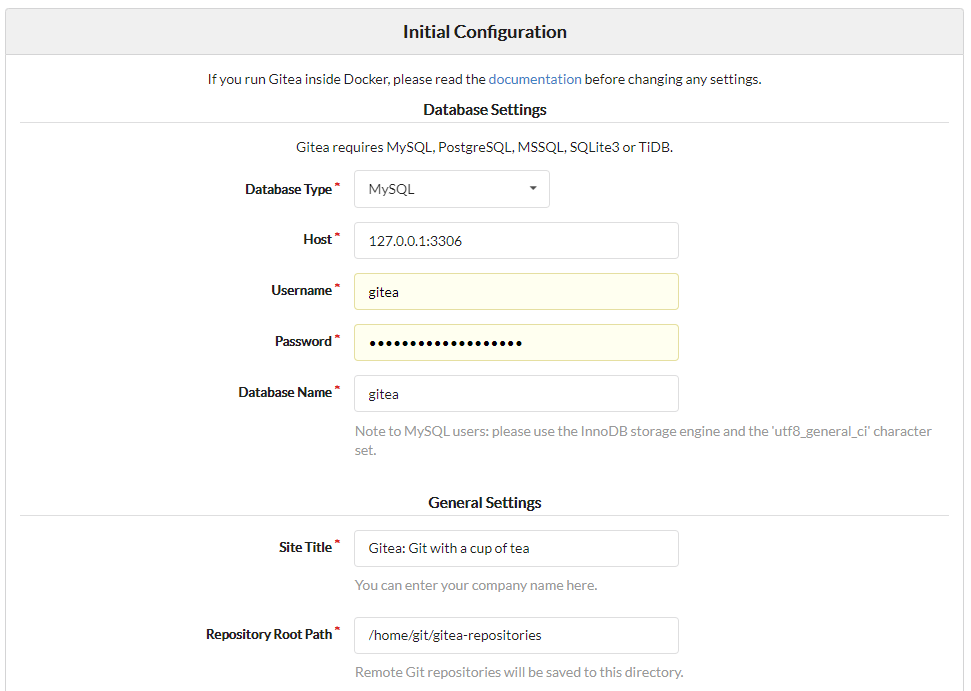
\includegraphics[width=0.8\textwidth]{images/initial_conf.png}
    \caption{Gitea setup page}
    \label{fig:gitea-setup}
\end{figure}
To avoid this, the deployment is provided with two things.

\textbf{First} is the \javaf{app.ini} file, which is the configuration file for Gitea. If no \javaf{app.ini} file is provided, 
it will be populated with data from the initial configuration page. The \javaf{app.ini} file is located in \javaf{src/gitea/config/app.ini}.

\textbf{Second} is a minimal installation of Gitea. This minimal installation is found in \javaf{src/gitea/config/gitea.tar.gz}. 
It is a simple setup of Gitea that, after the initial configuration, takes only a minute to set up. By placing the \javaf{gitea.tar.gz} file in the container 
directory \javaf{\data}, the Gitea instance will be set up with this minimal installation.
After initialization of Gitea, the script \javaf{src/gitea/start.sh} is run.
The script will curl the Gitea application to wait until Gitea is running.
The script will create \javaf{users}, \javaf{tokens}, \javaf{webhooks}, \javaf{Oauth} and \javaf{Oauth_grant}.
The script collects the information about these things from \javaf{src/gitea/config/}.

\subsection{Drone}
\label{sec:pipeline-local-drone}
Drone uses a script to initialize all the infrastructure supporting the pipeline and the underlying \ac{CTF}'s. 
Typically, when the drone is initialized, it contains no users or information about repositories. However, for a localized pipeline, 
it would be highly advantageous to have repositories and users present before the users first log in to the pipeline.

The initialization script for Drone resides in \javaf{src/drone/init.sh}. 
Since there is no direct access to the Drone data before the actual program starts through the 
\ac{API} or \ac{CLI}, a database.sql file is created, manipulated, and fed to the Drone container.
Drone utilizes a SQLite database, and data is inserted into the database using \javaf{sqlite3} commands. 
An example of a command used to insert users into the Drone database is depicted in Figure \ref{fig:sqlite3-insert}. 
The complete script can be viewed in the source code.

\begin{figure}
    \begin{center}
        \javaf{sqlite3 /data/database.sqlite "INSERT INTO users"}
    \end{center}
    \caption{sqlite3 command to insert users into the drone database}
    \label{fig:sqlite3-insert}
\end{figure}

To create and define these users and repositories before the drone program starts, 
they must match exactly on the Gitea side. 
Drone utilizes configuration files from the \javaf{src/drone/config/} 
folder to create the users and repositories. The configuration data in these \ac{CSV} files are identical to those used to create users and push repositories to Gitea.

\subsection{Nginx proxy}
\label{sec:pipeline-local-nginx}

Whenever a user interacts with the infrastructure, it will 
request by \ac{DNS} record to the gateway of the Docker Network, nginx reverse proxy, when then pickup that request, and 
proxy it to the correct container. The reverse proxy is also located inside a container, and is able through the Docker network,
to communicate with other containers. If another container outside the \javaf{docker network}
would like to communicate with a application inside the network, it would have to
go through the reverse proxy.

As described in section \ref{sec:nginx}, the reverse proxy is configuration is located in \javaf{src/proxy/default.conf}.
The conf file has three server blocks which includes the \javaf{ssl_certificate}, \javaf{ssl_conf}, and the \javaf{proxy_pass}.
These three things define what the reverse proxy does whenever a user calls the DNS record. The \ac{DNS} record for a 
specific server block is defined as \javaf{server_name}. The configuration for the proxy pass to Gitea is shown in Figure \ref{fig:nginx-proxy-pass}.

\begin{figure}[h]
    \centering
    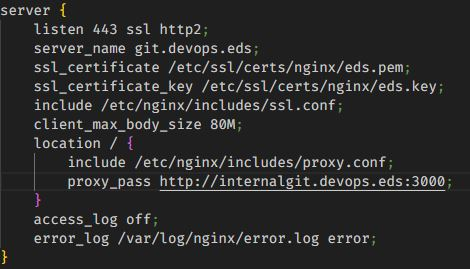
\includegraphics[scale=.7]{images/git_proxy_pass.jpg}
    \caption{Nginx proxy pass to Gitea}
    \label{fig:nginx-proxy-pass}
\end{figure}

\subsection{Docker}
\label{sec:pipeline-local-docker}
Docker serves as the backbone of the pipeline, facilitating easy deployment, maintenance, and development. 
Leveraging Docker as the containerization tool enables deployment and utilization across various environments. 
The Docker containers are specified in the \javaf{docker-compose.yml} file, located within the \javaf{src} directory.

Docker will spawn five containers and attach itself to the Docker network, when the \javaf{prerun} script is run.
\javaf{Nginx}, \javaf{Gitea}, \javaf{Drone}, \javaf{Registry}, and \javaf{Drone-runners}.
Whenever the pipeline is spawned Docker will create new images. This is to make sure that, if new changes are made 
that they are included in the new run. Docker can sometimes force itself to use cached images instead of building new 
ones if the changes are small.

The configuration for the pipeline all relies in the \javaf{docker-compose.yml} file. If any of the link, volumes, network etc. 
is wrongly configured, the pipeline might run, but it might mean that a CTF or a webhook will not create the desired outcome.\\
Differently from the remote pipeline, in the localized pipeline, Gitea and Drone are supplied with the Oauth2 application and Oauth2 grant
before it is initialized. 
By doing so, the user will not have to go through the initial setup of the application and will have access 
right away to Drone without having to authenticate through Gitea.

\subsection{Registry}
\label{sec:pipeline-local-registry}
As the project needed a local registry to fetch and push images into, the registry is a crucial part of the pipeline.
The registry used is developed by Distribution.\cite{registry}
The registry is a image registry similar to DockerHub, although DockerHub is actually isn't a registry, but a 
frontend to view available images. 
Typically, when users use the \javaf{docker pull} command, images are fetched from DockerHub. 
However, when utilizing a local registry, ensuring that images are pulled from it requires specific steps. 
The container hosting the registry must include a designated \javaf{certs} folder to inform Docker that the local registry, 
which employs a self-signed certificate, is a trusted source.\\
To establish trust in the untrusted registry mirror, the certificate must be placed in the root Docker configuration folder, specifically in \\ 
\javaf{/etc/docker/certs.d/}, with the URL of the registry, in this case, being \\
\javaf{registry.devops.eds}.
Then whenever a users or a runner wants to pull an image from the registry, it will have to use the specific URL.
see figure \ref{fig:specific_registry_url} for 
an example of a image pull in a pipeline.\\
\begin{figure}
    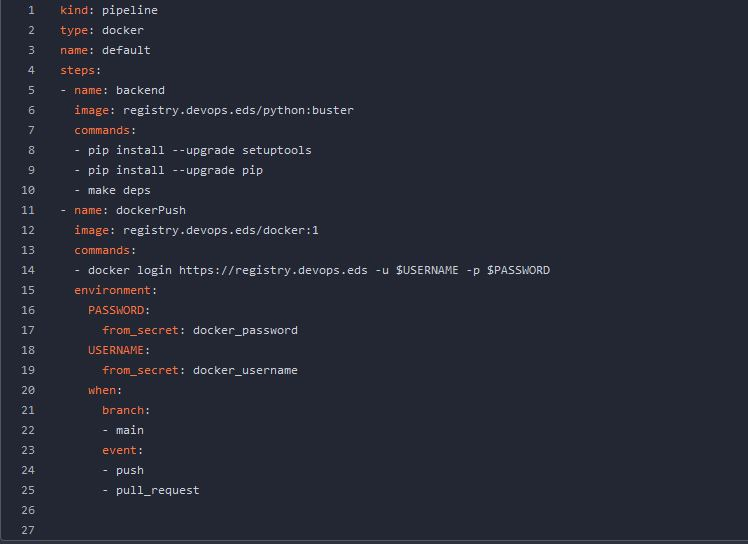
\includegraphics[scale=0.65]{images/local-registry-pull.jpg}
    \caption{Pulling an image from the local registry}
    \label{fig:specific_registry_url}
\end{figure}
The local registry work just like \url{https://registry-1.docker.io}. Although it different from \url{https://hub.docker.com}
. DockerHub is the a UI to find version and images, but isn't the actual registry where the images are stored.

\subsection{Certificate}
\label{sec:pipeline-local-certificate}
In the pipeline, a self-signed certificate with a Certificate Authority (\ac{CA}) is 
utilized to ensure security. This certificate is then distributed to all containers, 
ensuring uniform usage. It facilitates secure communication over HTTPS within the infrastructure, specifically with the \ac{TLD} starting with 
\javaf{*.devops.eds}. Details regarding the creation of this certificate are addressed in Section \ref{sec:certificate}.
\newpage

\section{\ac{CTF}}
\label{sec:ctf}

\subsection{Training repository for Drone}
The knowledge of pipeline configuration is essential in order for a developer to understand how to configure a pipeline.
As there are many pipeline tools and software, the knowledge of the specific pipeline tool is essential.
In this CTF, the user is added to the repository Firelands.
Firelands runs the user through how to construct a pipeline in Drone. The training material comes in five steps:
\begin{itemize}
    \item Step 1 - Pipeline kind, type, name.
    \item Step 2 - Using a steps - Executing a command on a runner.
    \item Step 3 - Using a services, hence a database or a web server.
    \item Step 4 - Using second steps after the first.
    \item Step 5 - Using environment variables and secrets in the steps part.
\end{itemize}

Introducing these parts of the Drone pipeline allows the user to understand and know how 
the pipeline works before delving into the CTF's. A complete solution for the first CTF or training repository can 
be see in \ref{app:firelands-solution}

\subsection{Remote code execution, on a runner}
For pipelines today, execution of code is of great importance. It leaves computational tasks to runners, which normally resides 
on a different machine than the users. That is a good practice, since it leaves the user machine free to focus on quick
development and will not use any computing power on running code. But this also leaves the runner open to attacks.

When using pipelines, the runners execute whatever the pipeline configuration tells it to do without any questions.
In most of the cases, the execution phase is smooth and without any problems, but what if the pipeline is compromised?

\paragraph{Amirdrassil repository\cite{photoview} - Remote code execution CTF's}
In the CTF's a new developer is given access to an already developed project. 
The developer becomes part of the Amirdrassil project 
and is left will all the possibilities to change and execute the pipeline by pushing code to the repository. The developer 
must take control of the pipeline eq. the runners and execute code on the runner to grab the flag. 
The solution to the pipeline can be found in \ref{app:amirdrassil-solution}.

\subsection{Stolen Credentials}
\label{sec:stolen_credentials}
Credentials are the keys to the kingdom. Credentials are essentials to security, since is something really secure if there is no 
way to access, then it might just be classified as inaccessible and not secure. Credentials are a crucial part of a security chain in a 
system. If credentials are stolen, all other security measures are useless.

In todays world of \ac{devops}, accessing remote or internal systems is done by credentials.
Drone handles the credentials either per repository or per organization. Drone does not specify how the secret are stored,
but after a look into the database of Drone, it seems they are stored in clear text in the database. 
it is uncertain whether they are protected by a layer of security measure or not.
However, accessed by the runner with a simple linux command such as \texttt{echo \$\{SECRET\}}, shows the asteriks representation of 
the secret is printed out in the logs.

What this means, if the runner is compromised, the credentials is still safe since the runner does not reveal the secret when printed to stdout.
For the solution to this CTF, the developer takes control of the pipeline. Then changes the pipeline to access secrets stored on the runner and 
print them out in clear text. See solution for the pipeline configuration can be seen in appendix \ref{app:amirdrassil-solution}.

\paragraph{Abberus repository\cite{flask-foundation} - Steal credentials CTF's}
To simulate an attack where an attacker steals secret credentials used to access a registry, consider the following scenario:

The repository simulates a typical organizational repository, with the pipeline defined in the .drone.yml file. 
This pipeline represents the usual steps for executing tasks on either a test branch or the main branch. 
The attacker, positioned as a developer, faces restrictions such as branch protection on the main branch and a repository webhook that triggers only on push events and merge requests related to the main branch.

To steal the credentials, the attacker must navigate these constraints by leveraging their developer access to 
introduce malicious code or configurations within the scope of their permissions, 
thereby exfiltrating the credentials during a legitimate pipeline execution.
\begin{itemize}
    \item First, create a new branch. The name of the challenge is not important.
    \item After the branch has been created, the attacker must change the already constructed pipeline to print out the secrets.
    Drone protects the secrets by changing them to asterisk representation.
    To get the secrets in clear text, the attacker can create a command that changes the secret into another string than the secret.
    \begin{center}
        \javaf{- echo $(echo $PASSWORD | sed 's/./&w/g' | sed 's/w//g')}
    \end{center}
    \item When the attacker has changed the pipeline, the attacker then creates a merge request to the main branch,
    which will trigger the pipeline to run the changed pipeline.
    \item Last the attack copies the changed string to the host pc and removes the extra character that was added.
\end{itemize}

An entire solution of the pipeline can be found in appendix \ref{app:abberus-solution}


\subsection{Supply chain attack}
\label{sec:supply_chain_attack}
A supply chain is when a user of a software program or software developer environment uses
third party, open source software or a other software to build or run their own software or environment.
Meaning that the program is dependent on another program to be bug free, secure, and reliable.

A project might not always use supply chain to run but based on the fact that more companies and developers are more prone to use 
third party software than ever, the risk of a supply chain attack is increasing. 
Information from various sources indicates that the risk of supply chain attacks is increasing. 
This rise is attributed not only to the growing number of third-party providers but also to the increasing number of compromised open-source projects.
\cite{supplychainbrain_supply_chain_breaches}\cite{statista_open_source_supply_chain_attacks}.

A supply chain attack occurs when third-party software is compromised. This software might be a dependency for another application or service.
 An attacker can alter or introduce a vulnerability into the third-party software. 
When the software is updated, the exploitable code becomes accessible, allowing the attacker to target the supposedly \texttt{"secure"} system.

Executing a supply chain attack is no simple feat. Typically, the attacker initiates the process with what is known as an upstream attack. 
In an upstream attack, the assailant targets the software or its provider directly. Once access to the software provider is obtained, 
the attacker may implant a vulnerability within the software. The subsequent phase of the supply chain attack involves the downstream attacker. 
Here, the downstream attack occurs when the newly implanted vulnerability is triggered within software that relies on the compromised software.
\cite{cloudflare_supply_chain_attack}

\paragraph{Ulduar and Icecrown repository - Supply chain attack CTF's}
The supply chain attack consists of two repositories, a repository were the user only has read access and another 
repository where the user has write access. 

\paragraph{Ulduar repository\cite{flask-blog}}
Ulduar is a repository where users have read-only access. It simulates a typical repository containing a pipeline file. 
This pipeline is configured on the drone server to run as a cron job every 2 minutes. 
Although it is uncommon for a pipeline to execute this frequently, it is set this way for simulation purposes to save time. 
The pipeline utilizes a Docker image, 
which is retrieved from the local registry created during the deployment of the entire infrastructure.

\paragraph{Icecrown repository}
In the Icecrown repository, the developer has full access. This repository simulates a supply chain for the Ulduar repository. 
Since the Ulduar repository uses a Docker image from the local registry, which Icecrown can access, it allows the developers to build a new, 
"infected" image within Icecrown's pipeline and push it to the local registry. When the Ulduar repository runs its pipeline, 
it will fetch and execute this new "infected" image. 
The user's task is to alter the Docker image used by the Ulduar repository so that the Ulduar repository prints out its flag.

\paragraph{Solution}
As this \ac{CTF} is not finished due to time constraints, the solution and general
source code is not complete. However the source code for the CTF and pipeline can be found under,\\
\javaf{src/gitea/repositories/Ulduar} and \javaf{src/gitea/repositories/Icecrown}.q


\chapter{HAAUKINS \& \ac{Ucloud}}

\section{\ac{Ucloud}}
\section{Ucloud - Infratructure as a Service (IaaS)}
\label{sec:ucloud}
The project's goal is to shed light on the security risks associated with using pipelines. 
Most IaaS providers, such as GCP, AWS, Azure, and others, entail significant costs. 
However, SDU is a partner in the recently launched Ucloud project, offering educators, professors, 
and students like myself affordable access to real computing power, potentially provided as a grant for research projects.

The operation of Ucloud differs somewhat from other IaaS providers. 
Despite being an IaaS provider, I'd like to provide an overview of IaaS, emphasizing its characteristics. 
Subsequently, I will delve into the unique aspects of how Ucloud functions and outline the distinctions 
between Ucloud and other IaaS providers.


\subsection{IaaS}
\label{subsec:iaas}
IaaS refers to a cloud computing service wherein the provider hosts 
infrastructure components typically found in an on-premises data center. 
These components include servers, storage, networking hardware, and the virtualization or hypervisor layer. 
The provider also offers various accompanying services, such as detailed billing, monitoring, log access, security features,
load balancing, clustering, and storage resiliency, encompassing backup, replication, and recovery (Source: \cite{iaas}).

Ucloud bears some resemblance to a conventional IaaS provider but exhibits distinct characteristics. 
The primary difference lies in Ucloud's focus on the university environment, 
deviating from a public-oriented approach and the development of traditional applications. 
Instead, Ucloud is designed for the utilization of computational power, akin to a regular IaaS, 
with a specific emphasis on research and education.

Given its tailored use for application development, 
Ucloud does not necessitate certain security measures that would be essential for a more public-facing IaaS.

\section{Ucloud and cloud infrastructure.}
\label{sec:ucloud}
For the project I decided that using the internal available cloud product ucloud would be sufficient, 
to deploy the pipeline. Thinking that Ucloud would be able to supply or atleast help me with the request I would 
have to create an infrastructure which relied on components spawned in docker images.

The first problem I encountered with Ucloud\cite{ucloud} was the allocating of funds. For me to able to have access to the 
computational power of ucloud they will have to grant me funds to be able to run their products. I dont have a problem with 
the need of funds to run machines, its the allocation process for student like me that is questionable at best.
When it comes to use of these machines things become very bureaucratical.
I had to start with already some funds that were allocated to me for being a \ac{CS} student at University of Southern Denmark.


The next problem was the nested virulization. Nested virtulization is important because, Ucloud will spawn 
a virtual machine, on there bare metal for me which i then get granted access to. Since I want to run docker images
i need to have access to the PID 1 on the given machines to have access the linux systemctl. If i don't
have access to PID 1, I wont be able to start the docker daemon and therefore not be able to run docker images.

Upon actualy being able to start working with Ucloud, the task of creating an infrastructure and using it publicly, was not as easy as I thought.
The first problem was that Ucloud does not have a product where i can upload my own docker images, and then deploy them.
I need to spawn machines and then run the docker image. Although this is not a huge problem, because actually 
having access to the machines that runs the docker images is actually kinda nice.

\subsection{Deployment and connection to Ucloud}
\label{subsec:deployment-and-connetion-ucloud}
\subsubsection{Deployment}
\label{subsubsec:deployment-ucloud}

Ucloud has different section of where you can deploy virtual machines. They are located at different universities around Denmark.
Those that are being used are mostly located at SDU and AAU. SDU instances has a single issues that makes that made them inenligible for
use and it's that they dont support nested virtualization. This is a problem, since the use of docker for the deployment of 
gitea and in general for the project is crucial, but more on docker in \ref{docker}

The AAU machines are spawned through the platform that ucloud supplies at \url{https://ucloud.aau.dk/}. How you spawn are machines is done 
in a couple of steps, first you need to figure what OS and version you want of that. Next name your instance and what type of 
virtual hardware you want. What was mostly used during the development of this project was 4 vCPU, 16GB RAM and 100GB disk.
The last thing before spawning the instance is supply an SSH-key, which is used to connect to the instance.

\subsubsection{Connection}
\label{subsubsec:connection-ucloud}
The connection to the instance is done through SSH. 
The SSH-key that was supplied during the spawning of the instance is used to connect to the instance. One of the main issues of the 
method of connetion is that there is no real possible for me to utilize the SSH connetion in a clever way. It is going to be done through 
port forwarding between multiple machines located inside the AAU-cluster network, and even then it's not possible for the machines 
to acutal be exposed to the internet as a web server. Because this is happening is becuase ucloud infrastructure is located behind a 
firewall, which is in front of the network called The Danish Research Network (Forskningsnettet). This is a network that is
used by all the universities in Denmark, and is used to connect them to the internet. The firewall is used to protect the
infrastructure from attacks from the internet. For this project, that is a problem, since the Gitea server will have to be publicly available 
for user to connect to it. 
The solution to this problem was solved by using Ngrok.

\subsection{Ngrok}
\label{subsec:ngrok}



\label{sec:ucloud}
\section{\ac{HAAUKINS}}
As discussed in Section \ref{sec:haaukins}, the absence of documentation and general feedback from the \ac{HAAUKINS} team
made it difficult to fully understand \ac{HAAUKINS} and its capabilities.
The intended use of \ac{HAAUKINS} in this project was to manage the infrastructure for the pipeline backend machines and handle flags.

Discussing the errors and issues that \ac{HAAUKINS} encounters during use is challenging because a 
thorough examination of \ac{HAAUKINS}, its features and structure was not been possible.
Consequently, conclusions about \ac{HAAUKINS} will be based on the information obtained 
from its minimal documentation, the GameSS project, and \ac{DDC}.\\\\
The future use of the \ac{HAAUKINS} program within the pipeline involves deploying 
it on an existing \ac{HAAUKINS} instance through the GameSS project. 
From there, CTFs will be integrated into the new pipeline.

Although the pipeline is not entirely new, it requires a fresh configuration for the \ac{HAAUKINS} platform to correctly spawn the backend containers, 
effectively making it a new pipeline. Additionally, because the \ac{HAAUKINS} platform uses specific DNS records, such as \javaf{hkn}, 
the certificate that enables \ac{HTTPS} communication between containers must be recreated to match the specific \javaf{.hkn} \ac{CN}.
\label{sec:haaukins}

\chapter{Discussion}
\label{sec:discussion}
As the need for pipeline security and automation grows, so does the demand
for educational and practice materials in these areas. While there may be
resources available for specific tools, there will always be a need for materials
or platforms that allow for practice in real-world scenarios. Therefore,
having the pipeline available on a local setup and having it available on \ac{HAAUKINS} 
will make the material for educational purposes more accessible.

\section{Ucloud}
\label{sec:discussion-ucloud}
\section{Ucloud - Infratructure as a Service (IaaS)}
\label{sec:ucloud}
The project's goal is to shed light on the security risks associated with using pipelines. 
Most IaaS providers, such as GCP, AWS, Azure, and others, entail significant costs. 
However, SDU is a partner in the recently launched Ucloud project, offering educators, professors, 
and students like myself affordable access to real computing power, potentially provided as a grant for research projects.

The operation of Ucloud differs somewhat from other IaaS providers. 
Despite being an IaaS provider, I'd like to provide an overview of IaaS, emphasizing its characteristics. 
Subsequently, I will delve into the unique aspects of how Ucloud functions and outline the distinctions 
between Ucloud and other IaaS providers.


\subsection{IaaS}
\label{subsec:iaas}
IaaS refers to a cloud computing service wherein the provider hosts 
infrastructure components typically found in an on-premises data center. 
These components include servers, storage, networking hardware, and the virtualization or hypervisor layer. 
The provider also offers various accompanying services, such as detailed billing, monitoring, log access, security features,
load balancing, clustering, and storage resiliency, encompassing backup, replication, and recovery (Source: \cite{iaas}).

Ucloud bears some resemblance to a conventional IaaS provider but exhibits distinct characteristics. 
The primary difference lies in Ucloud's focus on the university environment, 
deviating from a public-oriented approach and the development of traditional applications. 
Instead, Ucloud is designed for the utilization of computational power, akin to a regular IaaS, 
with a specific emphasis on research and education.

Given its tailored use for application development, 
Ucloud does not necessitate certain security measures that would be essential for a more public-facing IaaS.

\section{Ucloud and cloud infrastructure.}
\label{sec:ucloud}
For the project I decided that using the internal available cloud product ucloud would be sufficient, 
to deploy the pipeline. Thinking that Ucloud would be able to supply or atleast help me with the request I would 
have to create an infrastructure which relied on components spawned in docker images.

The first problem I encountered with Ucloud\cite{ucloud} was the allocating of funds. For me to able to have access to the 
computational power of ucloud they will have to grant me funds to be able to run their products. I dont have a problem with 
the need of funds to run machines, its the allocation process for student like me that is questionable at best.
When it comes to use of these machines things become very bureaucratical.
I had to start with already some funds that were allocated to me for being a \ac{CS} student at University of Southern Denmark.


The next problem was the nested virulization. Nested virtulization is important because, Ucloud will spawn 
a virtual machine, on there bare metal for me which i then get granted access to. Since I want to run docker images
i need to have access to the PID 1 on the given machines to have access the linux systemctl. If i don't
have access to PID 1, I wont be able to start the docker daemon and therefore not be able to run docker images.

Upon actualy being able to start working with Ucloud, the task of creating an infrastructure and using it publicly, was not as easy as I thought.
The first problem was that Ucloud does not have a product where i can upload my own docker images, and then deploy them.
I need to spawn machines and then run the docker image. Although this is not a huge problem, because actually 
having access to the machines that runs the docker images is actually kinda nice.

\subsection{Deployment and connection to Ucloud}
\label{subsec:deployment-and-connetion-ucloud}
\subsubsection{Deployment}
\label{subsubsec:deployment-ucloud}

Ucloud has different section of where you can deploy virtual machines. They are located at different universities around Denmark.
Those that are being used are mostly located at SDU and AAU. SDU instances has a single issues that makes that made them inenligible for
use and it's that they dont support nested virtualization. This is a problem, since the use of docker for the deployment of 
gitea and in general for the project is crucial, but more on docker in \ref{docker}

The AAU machines are spawned through the platform that ucloud supplies at \url{https://ucloud.aau.dk/}. How you spawn are machines is done 
in a couple of steps, first you need to figure what OS and version you want of that. Next name your instance and what type of 
virtual hardware you want. What was mostly used during the development of this project was 4 vCPU, 16GB RAM and 100GB disk.
The last thing before spawning the instance is supply an SSH-key, which is used to connect to the instance.

\subsubsection{Connection}
\label{subsubsec:connection-ucloud}
The connection to the instance is done through SSH. 
The SSH-key that was supplied during the spawning of the instance is used to connect to the instance. One of the main issues of the 
method of connetion is that there is no real possible for me to utilize the SSH connetion in a clever way. It is going to be done through 
port forwarding between multiple machines located inside the AAU-cluster network, and even then it's not possible for the machines 
to acutal be exposed to the internet as a web server. Because this is happening is becuase ucloud infrastructure is located behind a 
firewall, which is in front of the network called The Danish Research Network (Forskningsnettet). This is a network that is
used by all the universities in Denmark, and is used to connect them to the internet. The firewall is used to protect the
infrastructure from attacks from the internet. For this project, that is a problem, since the Gitea server will have to be publicly available 
for user to connect to it. 
The solution to this problem was solved by using Ngrok.

\subsection{Ngrok}
\label{subsec:ngrok}




\section{HAAUKINS}
\label{sec:discussion-haaukins}
As discussed in Section \ref{sec:haaukins}, the absence of documentation and general feedback from the \ac{HAAUKINS} team
made it difficult to fully understand \ac{HAAUKINS} and its capabilities.
The intended use of \ac{HAAUKINS} in this project was to manage the infrastructure for the pipeline backend machines and handle flags.

Discussing the errors and issues that \ac{HAAUKINS} encounters during use is challenging because a 
thorough examination of \ac{HAAUKINS}, its features and structure was not been possible.
Consequently, conclusions about \ac{HAAUKINS} will be based on the information obtained 
from its minimal documentation, the GameSS project, and \ac{DDC}.\\\\
The future use of the \ac{HAAUKINS} program within the pipeline involves deploying 
it on an existing \ac{HAAUKINS} instance through the GameSS project. 
From there, CTFs will be integrated into the new pipeline.

Although the pipeline is not entirely new, it requires a fresh configuration for the \ac{HAAUKINS} platform to correctly spawn the backend containers, 
effectively making it a new pipeline. Additionally, because the \ac{HAAUKINS} platform uses specific DNS records, such as \javaf{hkn}, 
the certificate that enables \ac{HTTPS} communication between containers must be recreated to match the specific \javaf{.hkn} \ac{CN}.

\section{Pipeline}
\label{sec:discussion-pipeline}
Two pipelines using the same programs were developed during this project.
One pipeline with a local Drone instance and a remotely connected Gitea server.
The other is a totally localized deployable pipeline with a local Gitea server and a local Drone instance.
For structural purposes, the pipelines are named \javaf{local} and \javaf{remote}.

\subsection{Local pipeline}
\paragraph{Configuration at initialization}
The local pipeline resolved all the issues encountered with the remote pipeline, 
but it required creating several configuration files for initialization. To ensure the pipeline deployment was fully automated, 
all infrastructure components such as users, repositories, webhooks, and secrets had to be set up before the first login to Gitea and Drone.
Since the setup had to be completed before the actual Gitea and Drone servers were running, manual insertion into the database was necessary. 
This meant that for creating secrets, users, webhooks, and other configurations, 
it was essential to insert the data into the databases of both programs. 
This process often led to large SQLite databases queries with incorrect data entries and unpredictable program behavior.\\
Testing the extensive configuration required running the pipeline and all related programs in Docker containers. 
Each configuration and deployment cycle took four to six minutes. Given that the deployment process for the 
localized pipeline was executed around 300-500 times.
\paragraph{Resource consumption}
As the pipeline used Docker to spawn runners inside a Docker image, the resource consumption 
could potentially be high at a point. Drone gives a restriction in how many runners a pipeline or project 
can run a the same time, but there is no restriction in how many Docker containers a runners can spawn to be able to 
complete its execution. This could potentially lead to a high resource consumption on the host machine.
To prevent this a quota for the runners could be set, but this was not implemented in the pipeline.
Because the quota wasn't implemented into the runners was because a thorough testing of computational resources 
and how much a runner would consume was not done during extreme load. However, it is uncertain whether, if implemented, 
this features should be something done in \ac{HAAUKINS} or something done directly into the pipeline. Implementing
would also mean for local deployment that overusing resources would not be a problem.

\subsection{Remote pipeline}
\paragraph{OAuth2 issue}
The remote pipeline was constructed to address an issue encountered with OAuth2. 
The problem arose because the Drone server and the Gitea server were both running on the same machine using the same URL, 
localhost, differentiated only by port numbers. This caused OAuth2 to malfunction, as it could not distinguish between the two servers, 
resulting in redirects to the wrong server and failed authentication attempts.\\
Through extensive testing and debugging, the solution was found to separate the two servers and assign a 
different URL to the Gitea server. This was achieved by deploying the Gitea server on a remote machine while keeping the drone server 
on a local machine. This allowed OAuth2 to differentiate between the two servers, leading to a successful authentication process.\\
Later in the thesis process, it was discovered that this 
issue could also be resolved on the same machine by using different URLs for the two servers and placing them behind a reverse proxy.
\paragraph{Pipeline structure}
In the remote pipeline setup, the Drone server was localized while the Gitea server was remote. 
This arrangement made the connection and communication between the two servers challenging. 
Normally, both the Drone and Gitea servers would be exposed to the internet. 
However, automating the exposure of the Drone server to the internet was not resolved.\\
To facilitate communication between the two servers, an SSH connection from the Gitea server machine 
to the Drone server was used. This allowed the Gitea server to send \javaf{GET, POST, DELETE, and PUT} requests through 
the SSH connection to the Drone server. This approach was necessary because the Gitea server resided in a VM on \ac{Ucloud}, 
and, as mentioned in section \ref{sec:connection-ucloud}, the VMs on \ac{Ucloud} are only accessible via SSH.
After the \javaf{drone.sh} script was completed, users had to manually create a key pair for the Gitea server, 
enabling it to establish an SSH connection and forward traffic to the Drone server.

Having this structure for the pipeline was not optimal. It had many 
drawbacks and wasn't really an automated deployment. There was almost issues with either 
creating users, webhooks, push repositories to remote Gitea, pipeline not being able to sync with the Gitea server,
Gitea not being able to communicate with the Drone server and so on.
\paragraph{Ngrok issue}
For having the Gitea remotely accessible Ngrok was used to create a public \ac{URL} to the 
server and exposing it. Although Ngrok offers free usage with a single domain, a change in the Terms of Service (TOS) 
limited the amount of data available to free users per month. This limitation rendered the pipeline unusable once 
the data quota was exhausted, making the remote Gitea server inaccessible. 
Consequently, Ngrok was abandoned, and the pipeline was moved to a localized solution.



\section{Reflections and improvements towards CTF's}
\label{sec:discussion-future-work}
Although the project is complete, the discussion has highlighted several problems and challenges encountered during its development. 
This reflection has made it clear that there are still areas that need improvement and further work in the future. 

\subsection{Last CTF, Supply chain attack}
As mentioned at the end of section \ref{sec:ctf}, the last CTF in development 
was not finished due to time constrains.
This CTF is likely one of the more challenging ones, both in terms of implementation and for the user to solve. 
Completing this CTF would have been a valuable addition to the pipeline.
Although some of the development aspects of the creating CTF's was challenging,
there were two main challenges that were unable to be achieved.
\paragraph{Cron Job, for timed execution}
Whenever creating a \javaf{Cron Job} for Drone the software, whenever creating it through the API or the CLI,
adds the next execution time based on whenever the \javaf{Cron Job} was created.\\
However, since the \javaf{Cron Job} was created by inserting it directly into the database, 
the software was not present to do next execution time calculation and therefore the insertion of a wrong format in the database makes the 
UI break for the \javaf{Cron Job} when viewed on the Drone UI.
\paragraph{Implementation a exploit through the Docker image}
The proposed solution for the \ac{CTF} challenge was to modify the Docker image used by Ulduar in its pipeline. 
This Docker image could be updated through another repository Icecrown, 
which had a pipeline containing credentials capable of altering the Docker image in the registry.
However, during the development of the \ac{CTF}s, 
it became clear that the Drone pipeline removes any commands or environmental variables inserted into the Docker image it uses. 
Consequently, without knowing if there is an exploit of this nature for the Drone pipeline, implementing an exploit for this \ac{CTF} proved difficult.

Therefore in the end, it was not achieved to implement this \ac{CTF} in the pipeline. 
The source code for the \ac{CTF} is available in the repository, and it is possible to implement it in the future.

\subsection{\ac{CTF}s on the pipeline}
In the end of the thesis, it was possible for the pipeline to be tested by real users. 
As for most of the project, it was only the author that tested, the feedback from the users was valuable.
Here is some of the feedback given, but all the feedback is included in the appendix \ref{app:feedback}.
\begin{itemize}
    \item \textbf{Amirdrassil} 
    One of the users had a difficult time, figuring out where the flag was located, because there 
    was not any mention or use of any kind of security aspect in the pipeline. The user 
    expressed that it would be an idea to change the password for one of the services used in the pipeline, to 
    use the an environmental variable which was the flag.
    \item \textbf{Firelands}
    Having a file named "flag.py" makes every user just go to that file and grab the flag. 
    The flag should be hidden better. The feedback gives a general sense of the training challenges missed its mark, 
    because the user can just grab the flag without solving the challenge.
    \item Another mentioned that instead of just handing over the credentials to the user account 
    on Gitea and Drone, the user should have to figure out how to get the credentials.
\end{itemize}

The feedback indicates that the challenges in the pipeline does work, but when gamifying
it, is important that there is only one way to solve challenges. When users does \ac{CTF}, they 
will always choose the fastest option to exploit or solve the challenge.

\chapter{Conclusion}
\label{sec:conclusion}

This thesis aimed to create a pipeline with 3-5 CTF challenges using \ac{HAAUKINS} and \ac{Ucloud}. 
The pipeline was built using Gitea, Drone, Docker, Nginx, Registry, and Docker Compose. 
It can be automatically deployed by any user on either Ubuntu or Kali Linux.

When incorporating \ac{HAAUKINS} and \ac{Ucloud} for the infrastructure, it became evident 
that using \ac{Ucloud} for the pipeline's computational power was not feasible. \ac{Ucloud}'s numerous restrictions, 
firewalls, and other security measures hindered control over the necessary resources, making its use impractical.

Regarding \ac{HAAUKINS}, it posed several challenges. My understanding of \ac{HAAUKINS} largely stemmed from the \ac{DDC} project. 
Initially, deploying the pipeline on \ac{HAAUKINS} was unachievable. Even after creating a localized solution, 
challenges remained due to network issues associated with \ac{HAAUKINS}, as discussed throughout the thesis. 
Additionally, after interacting with developers of HAAUKINS, it became clear that spawning HAAUKINS on \ac{Ucloud} was not possible. 
HAAUKINS requires access to the entire operating system to operate correctly, as discussed in section \ref{sec:discussion-haaukins}.

When comparing the two pipelines, it can be concluded that for CTF purposes, general use, 
and further development, a localized, self-deployed pipeline with Docker Compose is the best solution. 
The remote solution has some merit since it addressed the issue with OAuth2, but the problem with OAuth2 
was ultimately solved using a proxy and a \ac{TLD} in the localized pipeline.
However, the remote solution had too many flaws, 
including issues with SSH, SSH tunnels, webhooks, and the use of \ac{Ucloud} machines, which made it impossible to create any kind 
of smart communication between a local instance of Drone and a remote instance of Gitea.

With the use of a reverse proxy, it was possible for the \ac{CTF}s to be deployed locally. This meant that 
the \ac{CTF}s incorporated into the pipeline was able to be solved locally by anyone who deployed it.
The \ac{CTF}s in the pipeline are good, introducing Drone and providing general knowledge on how to interact with the pipeline. 

As the thesis was close to the end, the pipeline was tested by Brunnerne. That test proved 
that the pipeline was able to be deployed but other individuals than the author. 
From the feedback, it was clear that the pipeline was working as intended. 
The feedback mentioned that the challenges were nice, but they would like to see more technical challenges.

To summarize the thesis proposal, a pipeline incorporating CTF challenges was created. 
This pipeline is automated and can be deployed on the operating systems Ubuntu and Kali Linux. 
Regarding the use of \ac{HAAUKINS} and \ac{Ucloud}, we are currently planning to attempt deploying the pipeline 
on HAAUKINS after completing the thesis. However, due to numerous restrictions on machines in \ac{Ucloud}, 
utilizing \ac{Ucloud}'s computational power will not be feasible unless there are changes within its infrastructure. 
There is also potential for further development of CTF material for the pipeline based on 
feedback from Brunnerne, indicating room for improvement and additional content creation.

\label{lastpage} % Allows using the page number of this page as the last in 
% the footer
\newpage
\pagenumbering{gobble} % Stop numbering pages
\bibliographystyle{plain}
\bibliography{refs}
\rfoot{} % Remove page number from the footer

\appendix
\chapter{Appendix}
\newpage
\section{Certificate flag solution}
\label{app:certificate-solution}
\begin{minted}{bash}
    openssl s_client -connect git.devops.eds:443 -showcerts | grep "EDS"
\end{minted}
\section{Drone training CTF solution}
\label{app:firelands-solution}
\begin{minted}[
    gobble=4,
    frame=single,
    linenos]{yaml}
    kind: pipeline
    type: docker
    name: number1

    steps:
      - name: python1
        image: registry.devops.eds/python:buster
        commands:
            - pip install -r requirements.txt
            - python app.py
      - name: docker-using-environmental
        image: registry.devops.eds/docker:1
        commands:
            - sleep 3
            - docker login https://registry.devops.eds \
            -u $USERNAME -p $PASSWORD
            - echo "hello"
        environment:
          USERNAME:
            from_secret: USERNAME
          PASSWORD:
            from_secret: PASSWORD
      - name: flagtaking
        image: registry.devops.eds/python:buster
        commands:
          - python flag.py $FLAG
        environment:
          FLAG:
            from_secret: FLAG
    services:
      - name: python-server
        image: registry.devops.eds/python:buster
        commands:
          - python python_server.py
\end{minted}
\section{Peons will do what they are told solution}
\label{app:amirdrassil-solution}
\begin{minted}[
    gobble=4,
    frame=single,
    linenos]{yaml}
    kind: pipeline
    type: docker
    name: default
    steps:
    - name: backend
      image: registry.devops.eds/python:buster
      commands:
       - export | grep -E "EDS"
\end{minted}
\newpage
\section{Grab my credentials solution}
\label{app:abberus-solution}
\begin{minted}[
    gobble=4,
    frame=single,
    linenos]{yaml}
    kind: pipeline
    type: docker
    name: default
    steps:
    - name: backend
      image: registry.devops.eds/python:buster
      commands:
      - pip install --upgrade setuptools
      - pip install --upgrade pip
      - make deps
    - name: dockerPush
      image: registry.devops.eds/docker:1
      commands:
      - echo $(echo $PASSWORD | sed 's/./&w/g' | sed 's/w//g')
      environment:
        PASSWORD:
          from_secret: docker_password
        USERNAME:
          from_secret: docker_username
        when:
          branch:
          - mybranch
          event:
          - push
          - pull_request
\end{minted}

\section{Feedback}
\label{app:feedback}
\begin{longtable}{|p{0.15\textwidth}|p{0.25\textwidth}|p{0.10\textwidth}|p{0.40\textwidth}|}
  \hline
  \textbf{Date} g& \textbf{Title} & \textbf{Solved} & \textbf{Comments} \\
  \hline
  05-11-2024 13:05 & Empowering Devops Security - Code reviewing is important. & No & I think I've found unintended solve for this, Empowering Devops Security - Pipeline and Empowering Devops Security - Certificate
  
  Flags could all be read here: \url{https://git.imada.sdu.dk/mojak18/Empowering_DevOps_Security/src/branch/saturday-brunnerne/src/drone/config/secrets.csv} \\
  \hline
  5-13-2024 8:59:30 & Empowering DevOps Security & Yes & The information on where to look for a few of the challenges were a bit lacking, and the pipeline challenge could be solved by circumventing the challenge by reading flag.py. The setup was super intuitive and easy. The platform and challenges worked quite well \\
  \hline
  5-13-2024 13:56:41 & Empowering DevOps Security & Difficulty was fine & This challenge series is great for learning CI/CD, I enjoyed it. However, the flags for multiple challenges were visible directly in the source without solving the challenge.
  
  The Pipeline chall for instance seemed to be structured in a way where flag.py should have had only the hardcoded hash of the flag for verification - but the flag was visible directly in the code, so it wasn't even necessary to solve it. This seemed like a mistake since the code for checking against hash instead was already present. If fixing this, please make sure to alter the history of the repo, so the flag cannot be found in a previous commit.
  
  When gamifying learning in a CTF-style, it's really necessary that challenges cannot be completed without \textit{actually} solving them - people \textit{will} try to solve it the easiest way possible to get points/progress, even if this means not solving it in the intended way and missing out on learning. Nudging is important here, make sure flag isn't visible locally so people are forced to actually solve it.
  
  For the second and third repo, it wasn't clear to me, what the point was or what was meant to be done from the description and repo.
  
  But the idea was good and partially well executed! \\
  \hline
  05-11-2024 13:05 & Empowering Devops Security - Code reviewing is important. & No & I think I've found unintended solve for this, Empowering Devops Security - Pipeline and Empowering Devops Security - Certificate
  
  Flags could all be read here: \url{https://git.imada.sdu.dk/mojak18/Empowering_DevOps_Security/src/branch/saturday-brunnerne/src/drone/config/secrets.csv} \\
  \hline
  \end{longtable}
\printacronyms

\end{document}